 physical fitness test usually evaluates multiple components of one's health, including cardiovascular endurance, muscular strength, muscular endurance, flexibility and body composition.

In this chapter I will focus on familiarizing the reader with cardiovascular endurance testing, as it has the largest effect on hiking.
There is a number of indicators that one can measure (such as the lactate threshold - a non-linear increase in blood lactate concentration\cite{lactate-threshold}), 
but the most popular and easiest to measure with a heart rate monitor is VO2 max.

\section{VO2 and VO2 max}

The volume of consumed oxygen (VO2) is closely correlated with heart rate, respiration rate, and on/off-dynamics, all of which can be derived from RR interval data (time elapsed between two sucessive R waves -- the tallest spikes on an ECG),
with respiration rate being able to differentiate between metabolic (physical acitivity induced) and non-metabolic (mental and non-exercise related physical stress) changes in heart rate,
which makes models that take it into account highly accurate compared to those which only use heart rate.\cite{vo2-hr-firstbeat}

VO2 max, the maximal value of VO2, is considered the most accurate metric of cardiovascular fitness.

Measured in millilitres of oxygen consumed per minute or millilitres of oxygen per kilogram of bodyweight per minute, it is the amount of oxygen the body is able to effectively use (transform to energy) during intense or maximal exercise.
With the growing amount of oxygen the body can consume, it can perform better during strenuous activity and give improved results.\cite{vo2max-definition}
This is limited by the ability of the cardiorespiratory system to deliver oxygen to the exercising muscle, thus making it impossible for an athlete to operate above 100\% of their VO2 max for extended periods.\cite{vo2max-oxygen-delivery}

\begin{figure}[h]
    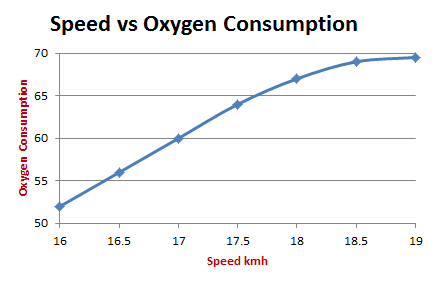
\includegraphics[width=\textwidth]{V02max-running.png}
    \caption{With increasing speed of the runner, oxygen consumption increases linearly and plateaus around 18.5 kilometres per hour - the VO2 max. \cite{vo2max-speed-img}}
\end{figure}

\subsection*{How to measure Vo2 max}

\subsubsection*{Laboratory test}

Typically, VO2 max is measured directly in laboratory conditions while wearing a respiratory mask, by analyzing inspired and expired breathing gases during maximal exertion,\cite{vo2max-definition} usually running on a treadmill or riding a stationary bike.

This method of determining VO2 max is highly accurate, but given the need for expensive equipment and trained staff, laboratory testing just isn't feasible for everyday population-wide testing.
On the other hand, results from laboratory tests are often used as reference values for determining the accuracy of alternative methods.

\subsubsection*{Cooper test - Twelve-Minute Run-Walk}

First suggested in the 1970's, Cooper's Twelve-Minute Run-Walk is an endurance test, where the main goal is to run (or walk) as long a distance as possible in twelve minutes.
It was originally developed mainly for armies and police agencies, but it's also popularly (and unnecessarily\cite{cooper-pupils}) used in schools on untrained pupils.
It is inaccurate for people who do not train running and swim or bike instead, as their bodies are used to a completely different set of movements.

There is a high correlation between the distance an individual can run and their VO2 max value, which can be calculated thusly:

$VO2max = (22.351 \times distance\_in\_kilometers) - 11.288$\cite{cooper-vo2max}

\subsubsection*{Multistage Fitness Test - Beep test}

Introduced by a Canadian sport scientist Luc Léger in the 1970's, this aerobic test has consistently been found a reliable way of finding a person's VO2 max.

The original version of the beep test (the Track Test) had the participants running back and forth in the interval of two minutes while the running pace was increased, so they always had to run further than in the previous iteration.

This test was highly efficient, however, given the long intervals and spatial requirements, it couldn't be performed indoors, giving rise to modifications, such as the Twenty-Metre Shuttle Run Test.
As the name suggests, two markers are placed twenty metres apart and again, the participants run back and forth between them, trying to reach the opposite marker before the next -- shorter -- stage begins, that is, before the next beep.
Once the test subject fails to reach a marker, turns without touching the marked line, or starts running before the signal, after one warning, their test is over.
They can also choose to stop when they have reached their maximum physical limit.

The test is divided into stages with recommended running speeds, each stage consisting of multiple shuttles - see the table at \cite{beep-test-scoring-table}.
From the stage and shuttle reached, one can calculate the VO2 max using the formula

\[VO2max (\frac{ml}{kg*min-1}) = 31.025 + 3.238X - 3.248A + 0.1536AX\]

where $A$ is age of the participant and $X$ is the speed in the final shuttle.
This formula fits the commonly used version of the Beep test (starting at 8.0 km/h, jumping to 9.0 km/h and continuing to rise by 0.5 km/h per level) and may vary depending on the version used.\cite{beep-test-versions}\cite{beep-test-20m-valid}

This modified version (just like the original) has been recognized as a valid method to determine VO2 max of male and female adults, individually or in groups, on most gymnasium surfaces.\cite{beep-test-20m-valid}

In 2017, Tomkinson et al. published a complex systematic study of nearly 1.2 million 9-17 years old children from 50 countries with data from beep tests as old as 1981,
setting standardized norms for testing of fitness in the world's youth.\cite{beep-test-youth-large-study}


\subsubsection*{Six-Minute Walk Test}

There are also some non-running tests which can be used to measure an individual's VO2 max.

The Six-Minute Walk Test, or 6MWT for short, originated from the Cooper test in the 1980's as a more feasible and less exhausting alternative.\cite{6mwt-history}

The main objective is for the participant to walk as long a distance as they can in the provided six minutes on a 15- or 30-metre long track, making sharp turns at the end.
Mänttäri et al. published a study in 2018\cite{6min-walk-test-mantarri}, aimed to develop a prediction model for VO2 max based on 6MWT results combined with heart rate at the end of the 6MWT and easy-to-measure anthropometric and demographic data (such as weight, height, age and gender).
The different track lengths only showed negligible differences between distances walked (on average, 23.5 m longer on the 30-m course).
\textit{For men, the best predictors for VO2max were walking distance, age, BMI, heart rate at the end of 6MWT and height, and for women, walking distance, age and weight} -- surprisingly, heart rate wasn't a significant factor for the female participants.

The formula they developed for men:

 $VO2 max=110.546 + 0.062\times distance - 0.25\times age - 0.486\times BMI - 0.42\times height - 0.109\times HR$

 and for women:

 $VO2 max=22.506 - 0.271\times weight + 0.051\times distance - 0.065\times age$

 \textit{where $weight$ is body weight (kg), $distance$ is distance walked in 6 min (m), $age$ (years), $BMI$ is calculated body mass index (kg/m2), $height$ is body height (cm) and $HR$ is heart rate at the end of the walking test (bpm).}

The authors themselves conclude that their output should be cross-validated with new independent samples of adult population,
but they consider it a precise enough method to be used for public health monitoring in adults.

Another study from 2015\cite{6min-walk-test-burr} instead used resting heart rate and arrived at this formula:

$VO2 max =70.161 + 0.023 \times distance - 0.276 \times weight - 6.79 \times sex - 0.193 \times resting_HR - 0.191 \times age$

using $distance$ walked during 6MWT (m), $weight$ (kg), $sex$ -- 1 for female, 0 for male, and $resting_HR$ for resting heart rate in beats per minute.

\subsubsection*{Sit-to-Stand test}

Another test that doesn't require much in terms of space or equipment and is in fact a common daily activity, which is often used to test lower body strength and endurance in older adults, has been studied for correlation with VO2 max values.
The Sit-to-Stand test, which consists of repetitive sitting down and standing up, has acquired a number of different forms just like most other tests used by the general public.
The versions include but aren't limited to the incremental twelve minute STS test -- sit and stand in incrementally shorter periods of time, repeated for twelve minutes, often controlled by a metronome \cite{seat-height-sit-to-stand};

Having been closely studied by Nakamura et al., it is a potentially valid test (when done with arm support, to increase the complete exhaustion threshold, and the right chair height, among other factors), but more research needs to be carried out to find a suitable version.\cite{frequencies-sit-to-stand}\cite{validity-sit-to-stand}

\subsubsection*{Non-exercise tests}

There are also some tests that do not require exercise and instead, have the individual fill out a questionnaire, such as the Jackson test\cite{nonexercise-vo2max-test-jackson} or the George test\cite{nonexercise-vo2max-test-george},
which ask questions on the topic of an individual's exercise habits, such as their perceived level of activity over the last six months.
Every answer has a specific weight in the resulting equation, based on which the person's fitness is evaluated.

These tests, however, should not be used as a sole source of information especially in medicine, as the data is self-reported and may be influenced by bias or conscious falsehood.

\section{The Performance Condition}

A person's VO2 max is recognized as their baseline fitness level index, however, everybody has days when they perform better, and days when they perform worse, while the factors in play are the amount of sleep they get, being sore from previous workouts, and general physical and mental wellbeing.

That is why Firstbeat introduced the Performance Condition.

Firstbeat is a provider of physiological analytics for sports and well-being who have translated human physiology into mathematical models based on heart rate variability (see below).
They provide their analytics engine as a service to a number of fitness device manufacturers, such as Garmin, Xiaomi, Honor and others.

The Performance Condition is a real-time index of a user's immediate fitness and fatigue level compared to their baseline fitness level.

This indicator is measured on a scale of -20 to +20, with each point representing roughly 1\% of their Vo2 max.
So if the user's current Performance Condition is +4, they can expect to perform outstandingly,
but at the same time, during the course of a workout, this number will decrease as fatigue from the exercise gets closer.\cite{performance-condition-firstbeat}\cite{performance-condition-garmin}

According to Firstbeat's support personnel, the formula behind the Performance Condition is protected information,
but generally, it uses a combination of personal background data, internal and external workload data, and special guidance from the Firstbeat analytics engine.\cite{firstbeat-performance-condition-emails}
Garmin's support website provides similar information: it is calculated based on the user's pace, heart rate and heart rate variability (HRV).\cite{performance-condition-garmin}

HRV is the variability in intervals between cardiac cycles.
It can be demonstrated, for example, by feeling one's pulse on the wrist while resting and breathing deeply - the interval shortens (heart beating faster) when breathing in, and lengthens (heart beating slower) when breathing out.\cite{hrv}
It's a complicated enough metric that to calculate it accurately, HRV should be measured using a chest strap,
an intrusive heart rate monitoring method which generally isn't available to a runner on a daily basis.

Additionally, the only activities that are currently supported for determining the Performance Condition, are running and cycling,
and the methods Firstbeat has developed to measure it has failed to satisfy a number of users, leading to them not paying much attention to the metric or outright ignoring the values.\cite{performance-condition-unreliable1}\cite{performance-condition-unreliable-reasoning}
One of the reasons behind their dissatisfaction is the fact that the metric only connects the effort the user is making with the distance they are covering,
 without taking into account the steepness of the slope, the humidity, temperature, and other external factors 
 and should be perceived more as an indicator of simply how much effort your body is making (as explained in BHerman's comment on a post\cite{performance-condition-unreliable-reasoning} in Firstbeat's forum), 
while being marketed as a highly precise metric that shows you how your training is going and not really explained well to the users.

\section{Heart rate zones}

Everybody has a resting heart rate (for example, right after waking up from a good night's sleep), and a maximum heart rate (the highest number of beats per minute achievable).
The range between HR min and HR max is commonly divided into five zones, based on the effort necessary and the effects the heart rate induces in a person:
\begin{itemize}
    \item Zone 1 (Warm up and very light exercise) --
    The trainee is relaxed at an easy pace and breathes rhytmically. Keeping one's heart rate in this zone helps with recovery from previous activities.
    \item Zone 2 (Easy, light exercise) --
    The trainee exercises at a comfortable pace, is able to hold a conversation and breathes slightly deeper. This zone is good for endurance practice.
    \item Zone 3 (Aerobic, moderate exercise) --
    At a moderate pace, it is more difficult to hold a conversation. Training in this zone helps improve aerobic capacity.
    \item Zone 4 (Threshold, hard exercise) --
    Training at a fast pace is somewhat uncomfortable, the trainee breathes forcefully. This zone is good for improving speed.
    \item Zone 5 (Maximum) --
    The trainee is at a sprinting pace, which is unsustainable for long period of time, and their breathing is laboured.
    This zone helps increase power in the trainee's body.\cite{garmin-heart-zones}\cite{polar-heart-zones}
\end{itemize}

Calculating HR min is an easy enough task - just measure your heart rate right after enjoying some good sleep; HR max is trickier.

\subsection*{Running methods to calculate HR max}
There are some methods to get HR max by running, such as running towards a hill at a high intensity and then ascending the hill at as high intensity as possible,
or, on flat ground, running 400 metres at high intensity and then increasing the intensity for another 400 metres.
These tests are considered stress tests, and individuals who are not highly active are not advised to take them. \cite{hrmax-running-tests}
Another method is based on interval running:
two intervals, four minutes each, in which the trainee is short of breath, interspersed by three minutes of active rest, and finished by a third interval, where two minutes in the trainee increases their speed as much as they can and run for as long as they can.
HR max is the maximum heart rate achieved.\cite{hrmax-running-tests-intervals}

\subsection*{Age-based methods to calculate HR max}
As the running methods are generally too difficult to do `on the spot', there have been attempts to calculate HR max based on readily available data.

The most commonly used formula to get one's maximal heart rate, $HRmax=220-age$ also known as the Fox formula, has been time and time again found largely inaccurate.
Originally intended as a rough formulation, with cross-sectional data from participants who are by no means representatives of a population\cite{220-hrmax-new-formula} and based on unoriginal research\cite{220-hrmax-disproved},
a number of researchers have tried to find a similarly simple but more accurate formulas, most of them claiming to have found the right one.
One of the popularly used is the cross-sectional research of Tanaka et al., who formulated the equation $208-0.7\times age$.
This formula was later validated by Gellish et al. in 2007 by conducting an analysis of longitudinal data from participants from various groups and developing a similar formula $207-0.7\times age$,
however, both Fox and Tanaka were disproved by Sarzynski et al. in 2014 as not precise enough based on standard error of estimate (12.4 and 11.4 bpm respectively) of the two formulas. \cite{hrmax-age-disproved}
In that study, Sarzynski stresses \textit{the importance of finding and validating other measures to be used in exercise prescriptions for the determination of intensity of exercise, the estimation of fitness levels, and as a criterion for achieving maximal exertion.}

The HUNT fitness study carried out on over three thousand people by Nes et al. found a more accurate formula $211-0.64\times age$, with the standard error of estimate of 10.8 bpm, but couldn't find evidence of interaction with gender, physical activity, VO2 max or BMI. \cite{hrmax-Nes-HUNT}


It seems that computational models for peoples' fitness leave a lot to be desired,
but this can all be remedied with further research.
